\documentclass[8pt,english,aspectratio=169]{beamer}
\mode<presentation>
{
  \usetheme{Pittsburgh}
  \usecolortheme{seagull}
  \usefonttheme{structurebold}
  \setbeamertemplate{navigation symbols}{}
  \setbeamertemplate{caption}[numbered]
}
\usepackage[utf8]{inputenc}
\usepackage[T1]{fontenc}
\usepackage[binary-units=true]{siunitx}

\usepackage{pgfpages}
\setbeamertemplate{note page}[plain]
\setbeameroption{show notes on second screen=right}
\usepackage[yyyymmdd]{datetime}
\renewcommand{\dateseparator}{--}
\usepackage{graphicx}
\usepackage{xcolor}
\usepackage{hyperref}
\usepackage{listings}
\usepackage{tikz}
\usetikzlibrary{positioning,arrows}
\tikzset{
block/.style={
  draw, 
  rectangle, 
  align=center
  }, 
line/.style={->,>=latex'}
}


\title[FVG Emergency Rooms situation]{FVG Emergency Rooms situation\\during Spring 2021\\\smallskip \small Data science project}
\author[\href{mailto:stefanel.enrico@spes.uniud.it}{Enrico Stefanel}]{Enrico Stefanel\\137411\\\href{mailto:stefanel.enrico@spes.uniud.it}{\texttt{stefanel.enrico@spes.uniud.it}}}
\date{\today}

\begin{document}


\begin{frame}
  \titlepage
\end{frame}

\begin{frame}{Data collection}
Friuli-Venezia Giulia region offers to the citizens the possibility to check live loads and average timings for every Emergency Room in the territory, thru the ``\href{https://servizionline.sanita.fvg.it/psonline}{Situazione nei Pronto Soccorso}'' web service, powered by \href{https://www.insiel.it/}{Insiel S.p.A.}.

Every 10 minutes since 2021-03-23, I run a Python script on my Raspberry Pi to collect this data and save it into a CSV file.

\medskip
\begin{center}
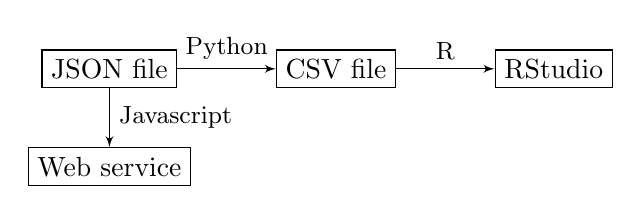
\begin{tikzpicture}
\node[block](a){JSON file};
\node[block, right=1.25cm of a](b){CSV file};
\node[block, right=1.25cm of b](c){RStudio};
\node[block, below=0.75cm of a](d){Web service};
\draw[line] (a.south) -- node[right] {\small Javascript} (d.north);
\draw[line] (a.east) -- node[above] {\small Python} (b.west);
\draw[line] (b.east) -- node[above] {\small R} (c.west);
\end{tikzpicture}
\end{center}
\bigskip

You can find the R Notebook of this project \href{http://uniud.enricostefanel.it/datascience/project/FVG_emergency_rooms_situation.html}{\color{gray}{at this link}}, and the raw dataset on \href{https://www.kaggle.com/enstit/friuli-venezia-giulia-emergency-rooms-situation}{\color{gray}{Kaggle}}.

\begin{block}{Disclaimer}
This study does not analyse COVID-19 situation in Friuli-Venezia Giulia: Emergency Rooms load is not a good index for COVID diffusion, since patients need treatments also for many other causes, such as domestic accidents, allergic manifestations, car crashes, \dots 
\end{block}

\note{Il mio progetto di \textit{Data Science} consiste nell'analisi delle presenze nei Pronto Soccorso della Regione dal 23 marzo ad oggi.

I dati sono stati raccolti in maniera automatica ogni 10 minuti, tramite uno \textit{script} Python che gira su un Raspberry Pi 4, e sono stati resi disponibili su Kaggle.

}
\end{frame}
\begin{frame}{Dataset}
The full dataset has three tables, but we only used two of them:

\begin{enumerate}
	\item \textbf{emergencyRooms}, that lists all Emergency Rooms in Friuli-Venezia Giulia, with relative address, healthcare company, notes, \dots; 
		\begin{center}\small
			\begin{tabular}{ |c|c|c|c|c|c|c| }
				\hline
				\textbf{emergency\_room} & \textbf{is\_pediatric} & \textbf{hospital} & \textbf{healtcare\_company} & \textbf{longitude} & \dots \\
				\hline
				\dots & \dots & \dots & \dots & \dots & \dots \\
				\hline
				\footnotesize Pronto Soccorso Cattinara & \footnotesize FALSE & \footnotesize Ospedale di Cattinara & \footnotesize ASU - Giuliano Isontina & \footnotesize 13.82627 & \dots \\
				\hline
				\dots & \dots & \dots & \dots & \dots & \dots \\
				\hline
			\end{tabular}
		\end{center}
	\item \textbf{attendances}, with records of Emergency Rooms loads every ten minutes, divided by priority colors;
		\begin{center}\small
			\begin{tabular}{ |c|c|c|c|c|c| }
				\hline
				\textbf{timestamp} & \textbf{emergency\_room} & \textbf{priority} & \textbf{examined\_patients} & \textbf{waiting\_patients} & \textbf{waiting\_time} \\
				\hline
				\dots & \dots & \dots & \dots & \dots & \dots \\
				\hline
				\footnotesize 1616454020000 & \footnotesize Pronto Soccorso Cattinara & \footnotesize Bianco & \footnotesize 2 & \footnotesize 1 & \footnotesize 02:36:00 \\
				\hline
				\footnotesize 1616454020000 & \footnotesize Pronto Soccorso Cattinara & \footnotesize Verde & \footnotesize 25 & \footnotesize 7 & \footnotesize 02:03:00 \\
				\hline
				\footnotesize 1616454020000 & \footnotesize Pronto Soccorso Cattinara & \footnotesize Giallo & \footnotesize 17 & \footnotesize 0 & \footnotesize 00:28:00 \\
				\hline
				\footnotesize 1616454020000 & \footnotesize Pronto Soccorso Cattinara & \footnotesize Rosso & \footnotesize 1 & \footnotesize 0 & \footnotesize 00:02:00 \\
				\hline
				\dots & \dots & \dots & \dots & \dots & \dots \\
				\hline
			\end{tabular}
		\end{center}
	\item \textbf{COVIDLocalRiskValuation} (unused in this studio), with local valuation of COVID situation, decided by the National Institute of Health (ISS).
		\begin{center}\small
			\begin{tabular}{ |c|c| }
				\hline
				\textbf{timestamp} & \textbf{risk} \\
				\hline
				\footnotesize 1614639600000 & \footnotesize high risk \\
				\hline
				\footnotesize 1618178400000 & \footnotesize medium-high risk \\
				\hline
				\dots & \dots \\
				\hline
			\end{tabular}
		\end{center}

\end{enumerate}

\note{Il dataset utilizzato era formato da tre tabelle:
	\begin{enumerate}
		\item \textbf{emergencyRooms}, che contiene l'elenco di tutti i Pronto Soccorso della Regione, con relative Aziende Sanitarie di appartenenza, indirizzo, eventuali note, \dots
		\item \textbf{attendances}, che è la tabella più corposa del dataset, e viene aggiornata ogni 10 minuti con il numero di pazienti sotto esame, in attesa e relativi tempi di attesa per ogni codice di priorità in ogni Pronto Soccorso della Regione. Allo stato attuale, questa tabella pesa circa \SI{50}{\mega\byte};
		\item \textbf{COVIDLocalRiskValuation}, che contiene l'elenco delle istituzioni delle varie aree di rischio nella Regione (zona rossa, zona arancione, zona gialla, zona bianca). È una tabella che ho aggiunto in un secondo momento, e che può essere utilizzata in maniera facoltativa per studiare se il COVID ha avuto un impatto significativo sul Sistema Sanitario regionale.
	\end{enumerate}

In questo studio i Pronto Soccorso pediatrici sono stati accorpati al Pronto Soccorso generale dello stesso ospedale, se esiste.

}

\end{frame}


\begin{frame}{Challenges}
Some questions we could ask about our scenario are, for instance:
\begin{enumerate}
	\item Which is the most used hospital?
	\item Is there any area in Friuli-Venezia Giulia that is poorly covered by Emergency system?
	\item Is \textit{waiting time} related to \textit{color priority}? If yes, how?
	\item How does Emergency Rooms entrance variate, during week days? Are there any days of week in which Emergency Rooms are more empty, compared to other days?
\end{enumerate}

\note{Prima di iniziare a lavorare sul dataset mi sono posto alcune domande:
\begin{enumerate}
	\item Qual è l'ospedale maggiormente utilizzato?
	\item Ci sono aree in Friuli-Venezia Giulia che sono scarsamente coperte dal Sistema di Emergenza Regionale?
	\item Il \textit{tempo di attesa} è correlato alla \textit{priorità}? Se si, in che modo?
	\item Come variano le presenze nei Pronto Soccorso durante i giorni della settimana? Ci sono alcuni giorni in cui i Pronto Soccorso sono mediamente meno affollati (ad esempio durante i fine settimana)?
\end{enumerate}
}

\end{frame}


\begin{frame}
In this map, every circle correspond to an Emergency Room. The color matches the Healthcare company which the Hospital belongs, and the size of the circle is proportional to the median of patients in the Emergency Room. Circles of Emergency Rooms with \texttt{NA} values for median load are semi-transparent filled.
\begin{figure}
  \centering
  \href{http://uniud.enricostefanel.it/datascience/project/images/map.html}{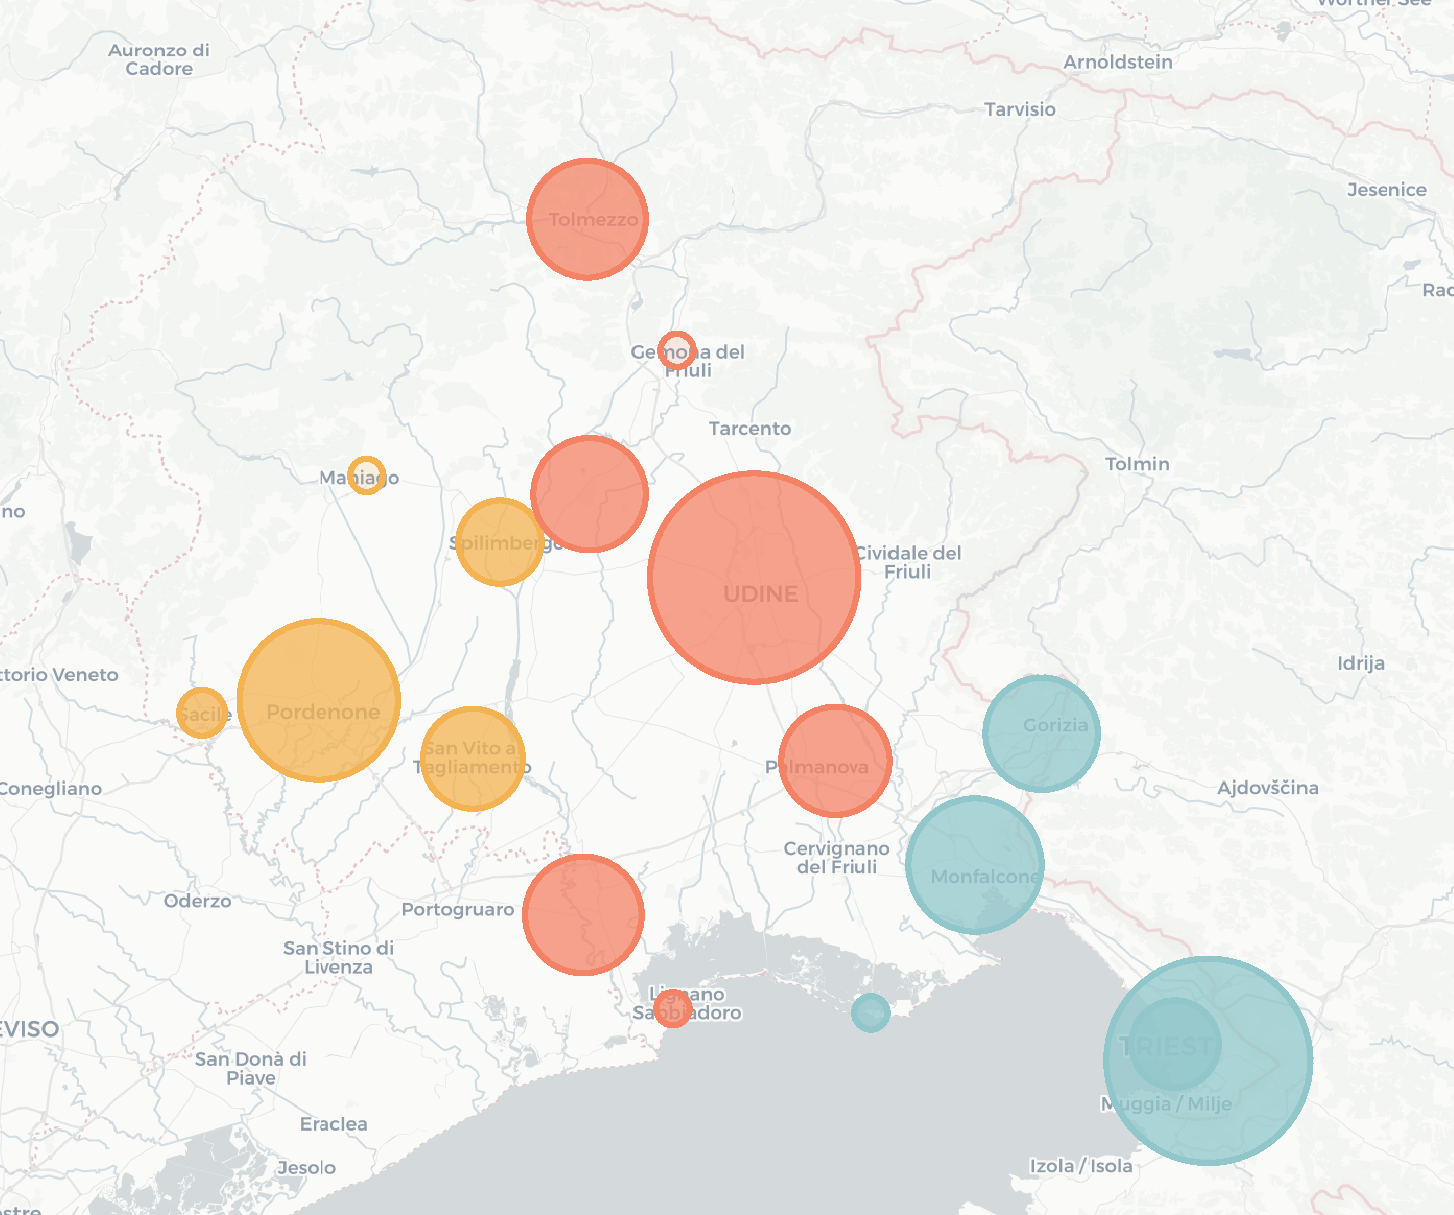
\includegraphics[width=0.75\textwidth]{../images/map.pdf}}
\end{figure}
\scriptsize \href{http://uniud.enricostefanel.it/datascience/project/images/map.html}{\color{gray}{Click}} on the map to open the interactive one.

\note{
\scriptsize Facendo \href{http://uniud.enricostefanel.it/datascience/project/images/map.html}{\color{gray}{click}} sull'immagine si apre la mappa interativa. \normalsize
\bigskip

Prima di tutto, ho visualizzato la localizzazione dei Pronto Soccorso sul territorio della regione.

Da questa mappa possiamo già notare alcune importanti proprietà:
\begin{enumerate}
	\item il colore corrisponde all'Azienda Sanitaria di appartenenza:
		\begin{itemize}
			\item in \textcolor{orange}{arancione}, l'\textit{AS - Friuli Occidentale} comprende gli ospedali che si trovano nel territorio dell'ex provincia di Pordenone;
			\item in \textcolor{red}{rosso}, l'\textit{ASU - Friuli Centrale} comprende gli ospedali che si trovano nel territorio dell'ex provincia di Udine;
			\item in \textcolor{blue}{blu}, l'\textit{ASU - Giuliano Isontina} comprende gli ospedali che si trovano nel territorio delle ex province di Gorizia e Trieste.
		\end{itemize}
	\item la dimensione del cerchio è proporzionale alla mediana del numero di pazienti che si trovano presso Pronto Soccorso in questione. Si nota già, come vedremo anche di seguito, che i Pronto Soccorso più numerosi sono quelli di Udine e Cattinara.
	\item alcuni cerchi sono semi-trasparenti (è il caso del Pronto Soccorso di Maniago e di Gemona del Friuli), perché sono chiusi a causa dell'emergenza da COVID-19.
\end{enumerate}
Notiamo che, nonostante il Pronto Soccorso di Tolmezzo sia l'unico Pronto Soccorso nella zona montana (che si estende per circa un terzo del territorio della Regione), non è tra i Pronto Soccorso maggiormente stressati.
}
\end{frame}

\begin{frame}
Now, we know the context. In the previous map, we could identify which are the Emergency Rooms with most patients, on average. Let’s visualize it with a \textit{boxplot}:
\begin{figure}
  \centering
  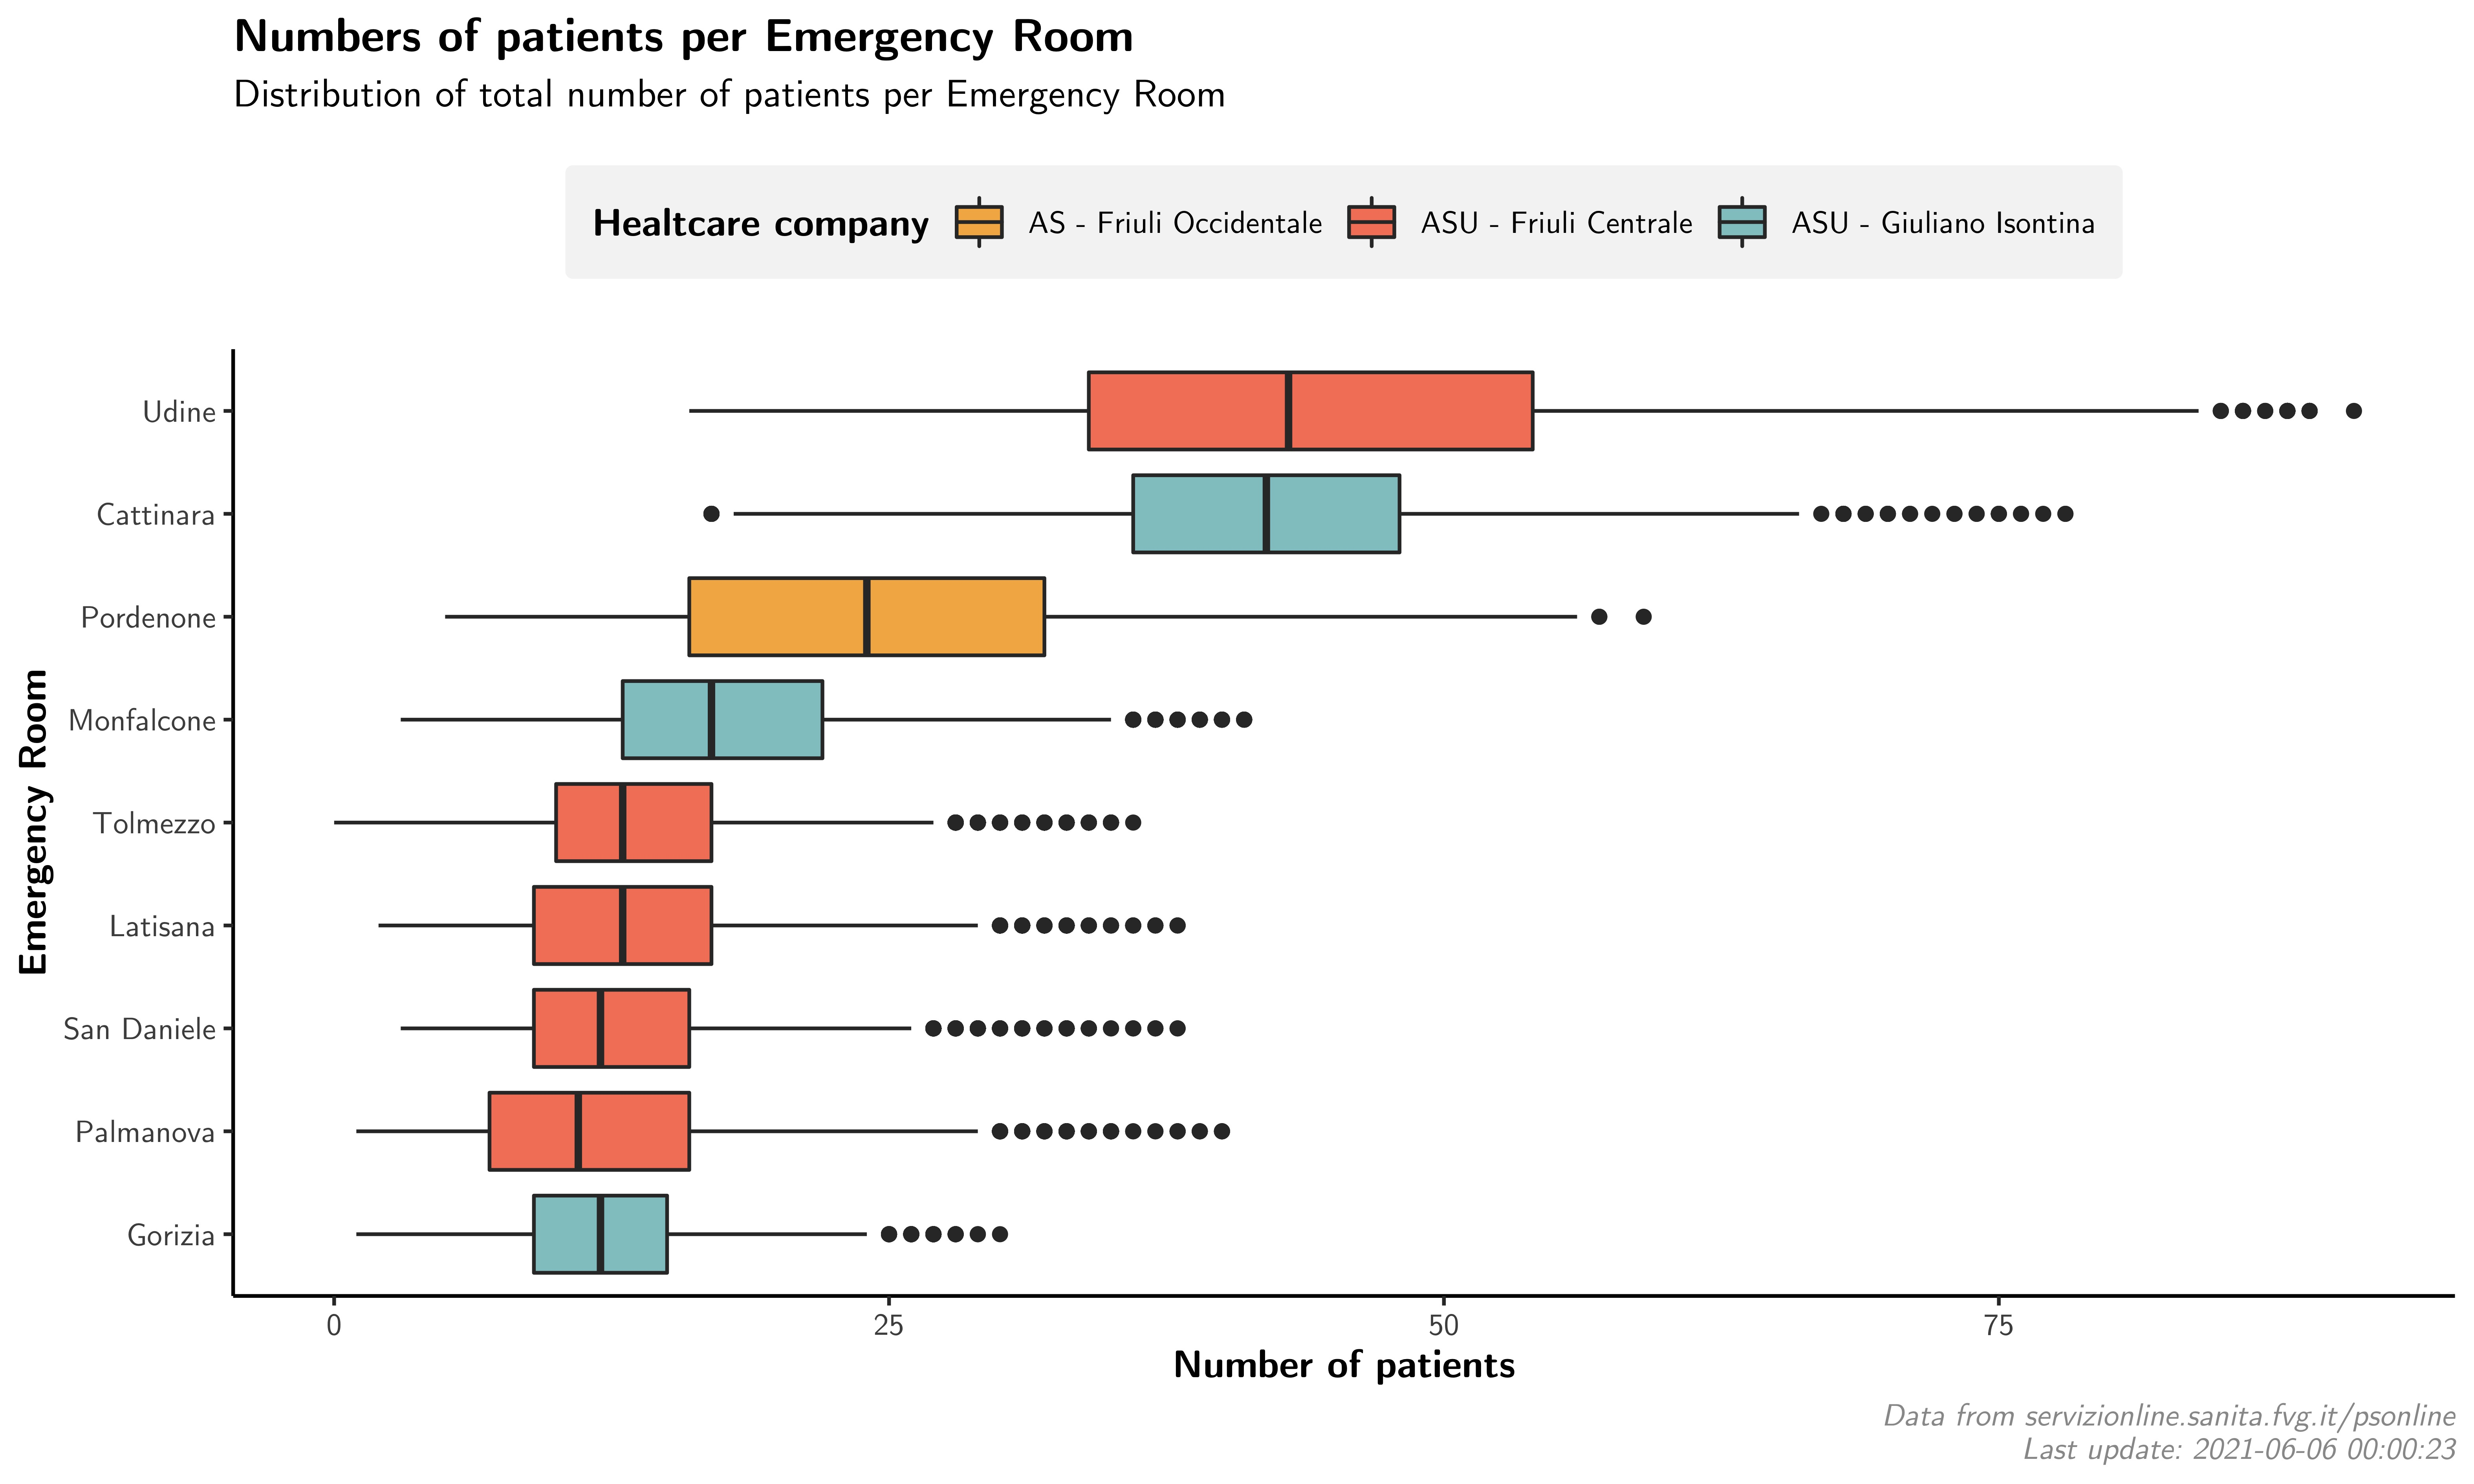
\includegraphics[width=0.75\textwidth]{../images/01_loads_boxplot.jpg}
\end{figure}
\note{Questo grafico con \textit{boxplot} ci conferma quanto avevamo già osservato nella slide precedente, ovvero:
	\begin{itemize}
		\item che il Pronto Soccorso di Udine è quello più ``frequentato'', ed inoltre notiamo che è anche quello con varianza maggiore;
		\item che il Pronto Soccorso di Cattinara è il secondo più ``frequentato'' dopo quello di Udine, mentre c'è un notevole distacco dai seguenti;
		\item i primi tre Pronto Soccorso, in ordine di saturazione, coprono tutti e tre le Aziende Sanitarie del territorio;
		\item i valori \textit{outliers} stanno tutti a destra della mediana, e in particolare tutti i \textit{baffi} sono più lunghi a destra che a sinistra. Questo significa che la singola distribuzione di presenze per Pronto Soccorso è sbilanciata verso sinistra;
	\end{itemize}

}
\end{frame}

\begin{frame}
\begin{figure}
  \centering
  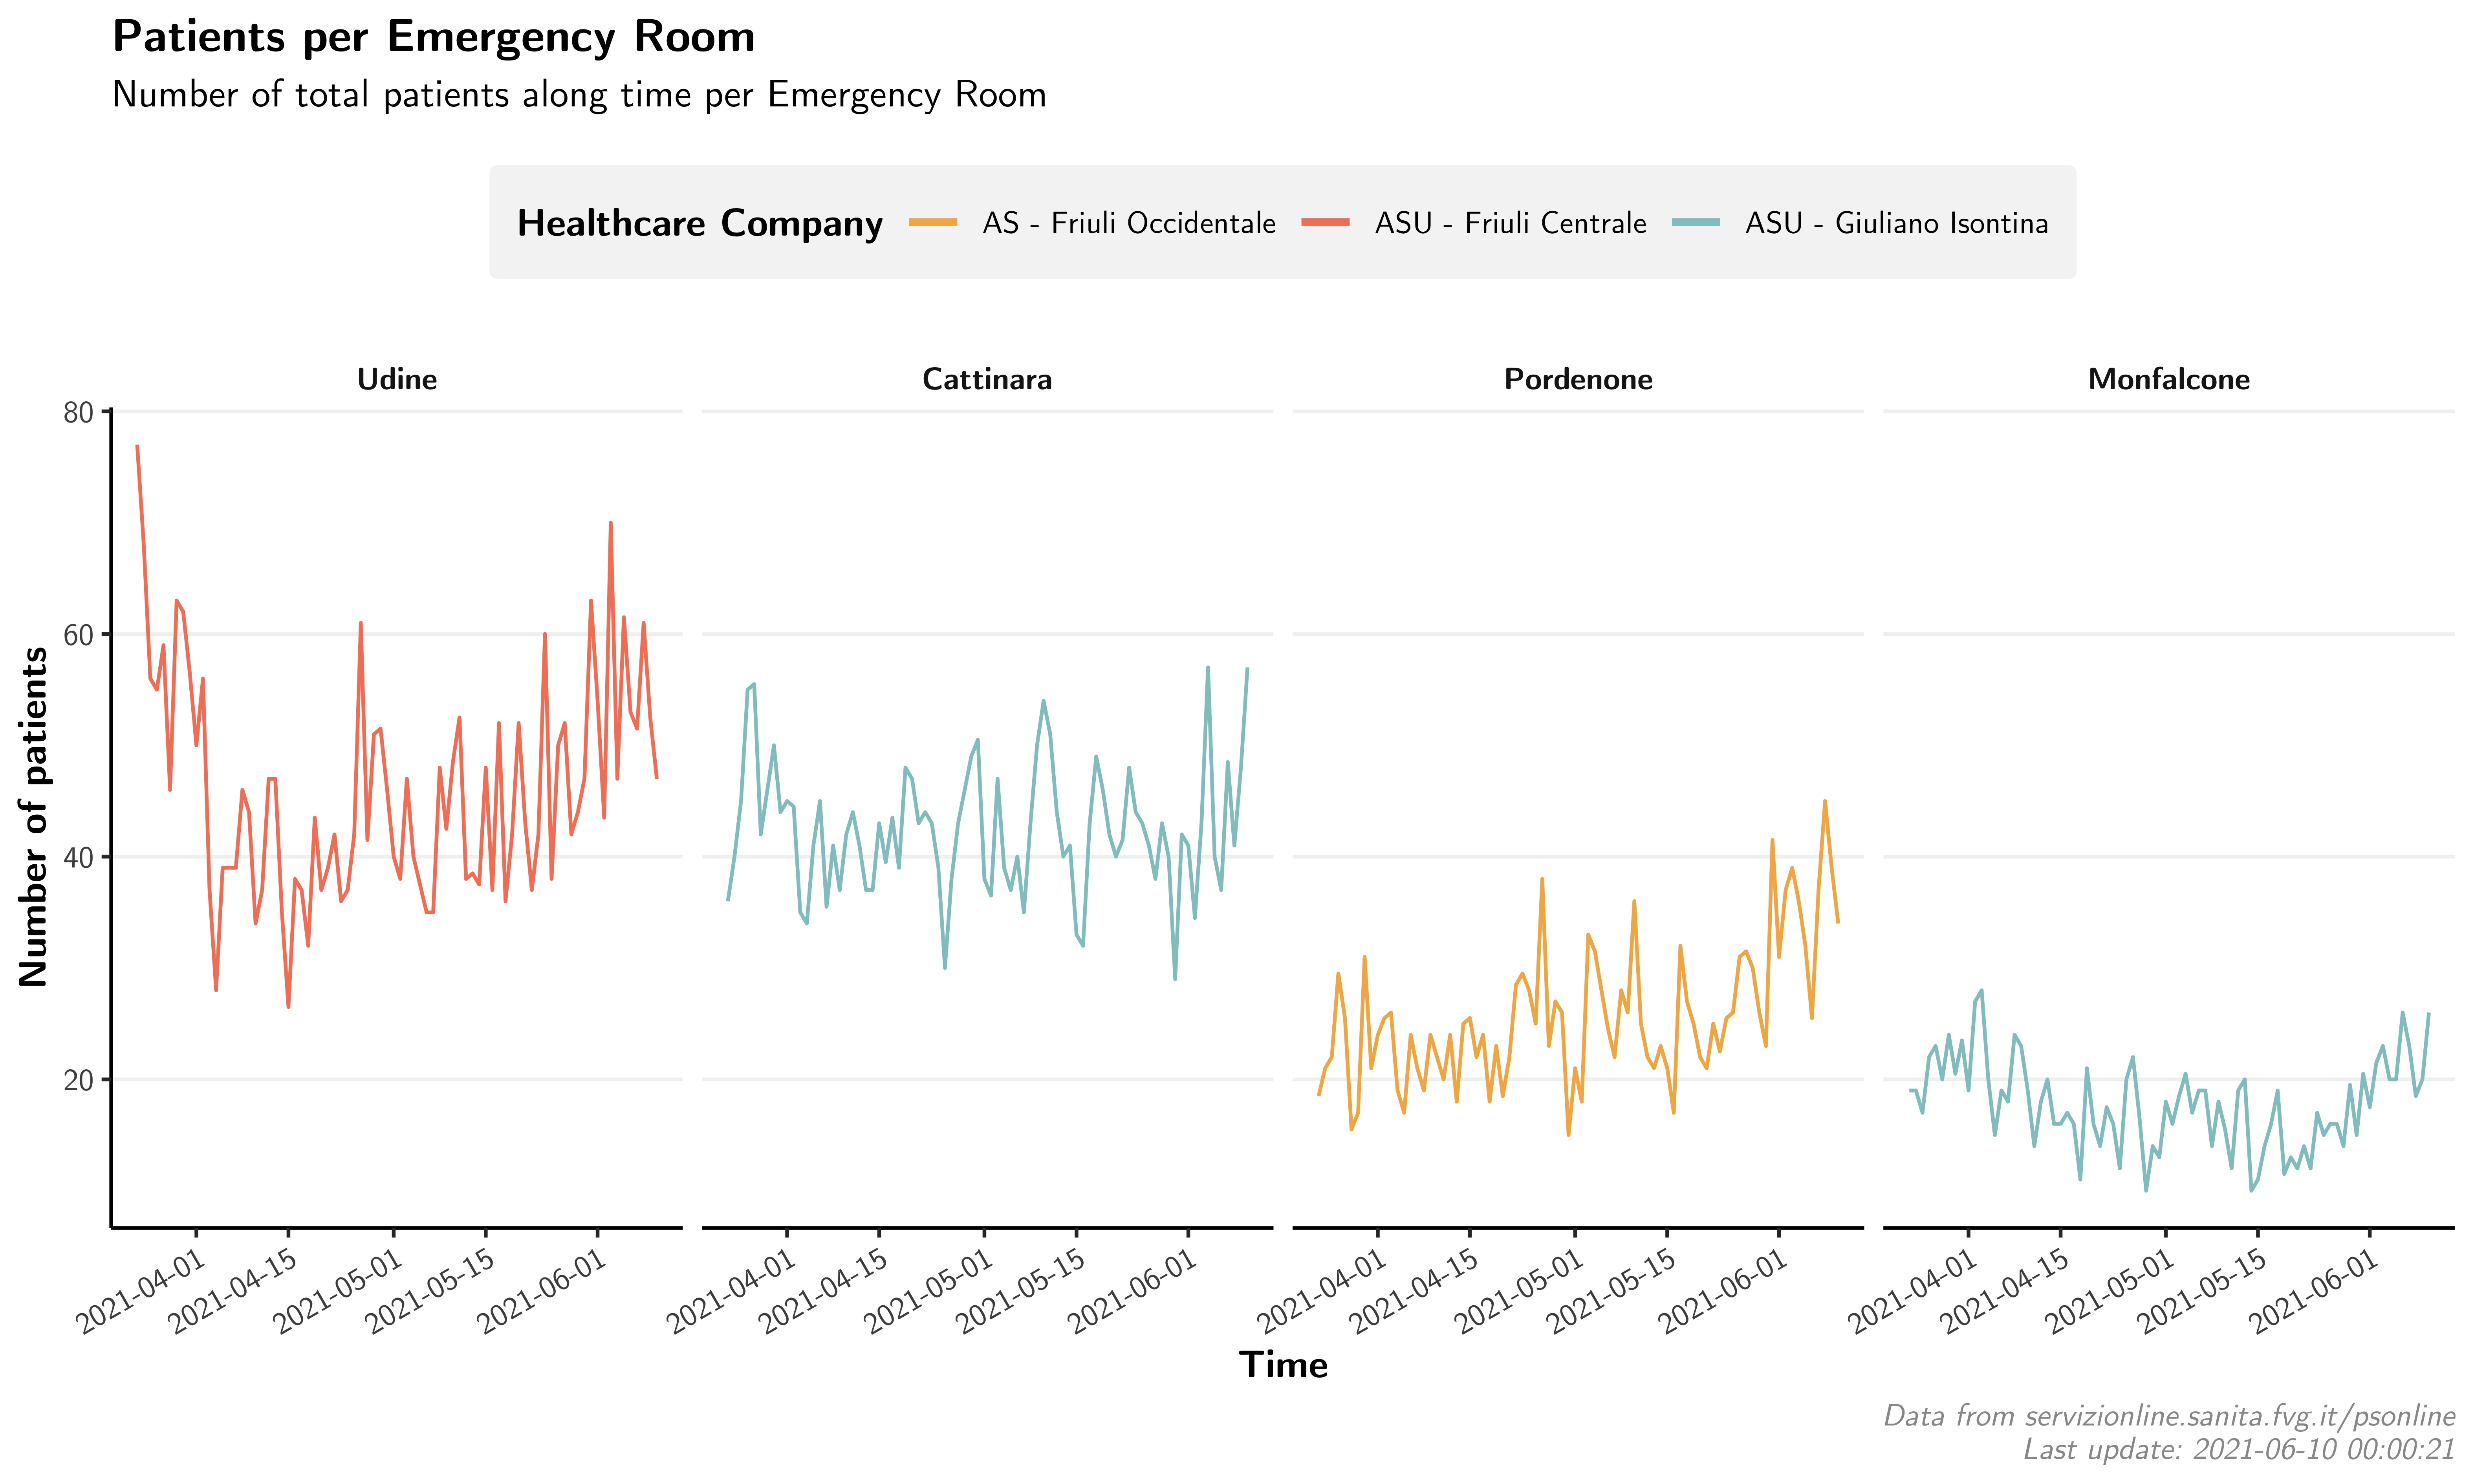
\includegraphics[width=0.75\textwidth]{../images/03_loads_trendlines-divided.jpg}
\end{figure}
\textit{Pronto Soccorso Udine} was very full on March, since it had almost the double of patients per day compared to first days of April in the same Emergency Room, but from April his trend is slowly increasing. \textit{Pronto Soccorso Cattinara} and \textit{Pronto Soccorso Monfalcone} trends are quite constant, while \textit{Pronto Soccorso Pordenone} average load is increasing.

\note{Questo grafico invece ci indica come sono variate le presenze nell'arco temporale dal 23 marzo 2021 ad oggi, relativo ai Pronto Soccorso con almeno 15 pazienti come mediana, ovvero quelli di Udine, Cattinara a Trieste, Pordenone e Monfalcone.
Il colore della linea indica l'Azienda Sanitaria di appartenenza.
}
\end{frame}

\begin{frame}
Our third question was ``How is color priority related with waiting time?''.
We could calculate \textit{Spearman} coefficient between the two variables, thinking priority as a discrete variable (from $1$ of 'Bianco' to $4$ of 'Rosso'):
\begin{center}\small
	\begin{tabular}{ c c }
		& \textbf{priority} \\
		\textbf{waiting\_time} & $-0.5005912$ \\
	\end{tabular}
\end{center}
The correlation has minus sign, so it is true that waiting time decrease when priority increase, as we were expecting. Although, the value of the correlation between priority code and waiting time is far from 1, describing a not-so-strong connection between the two variables.
\begin{figure}
  \centering
  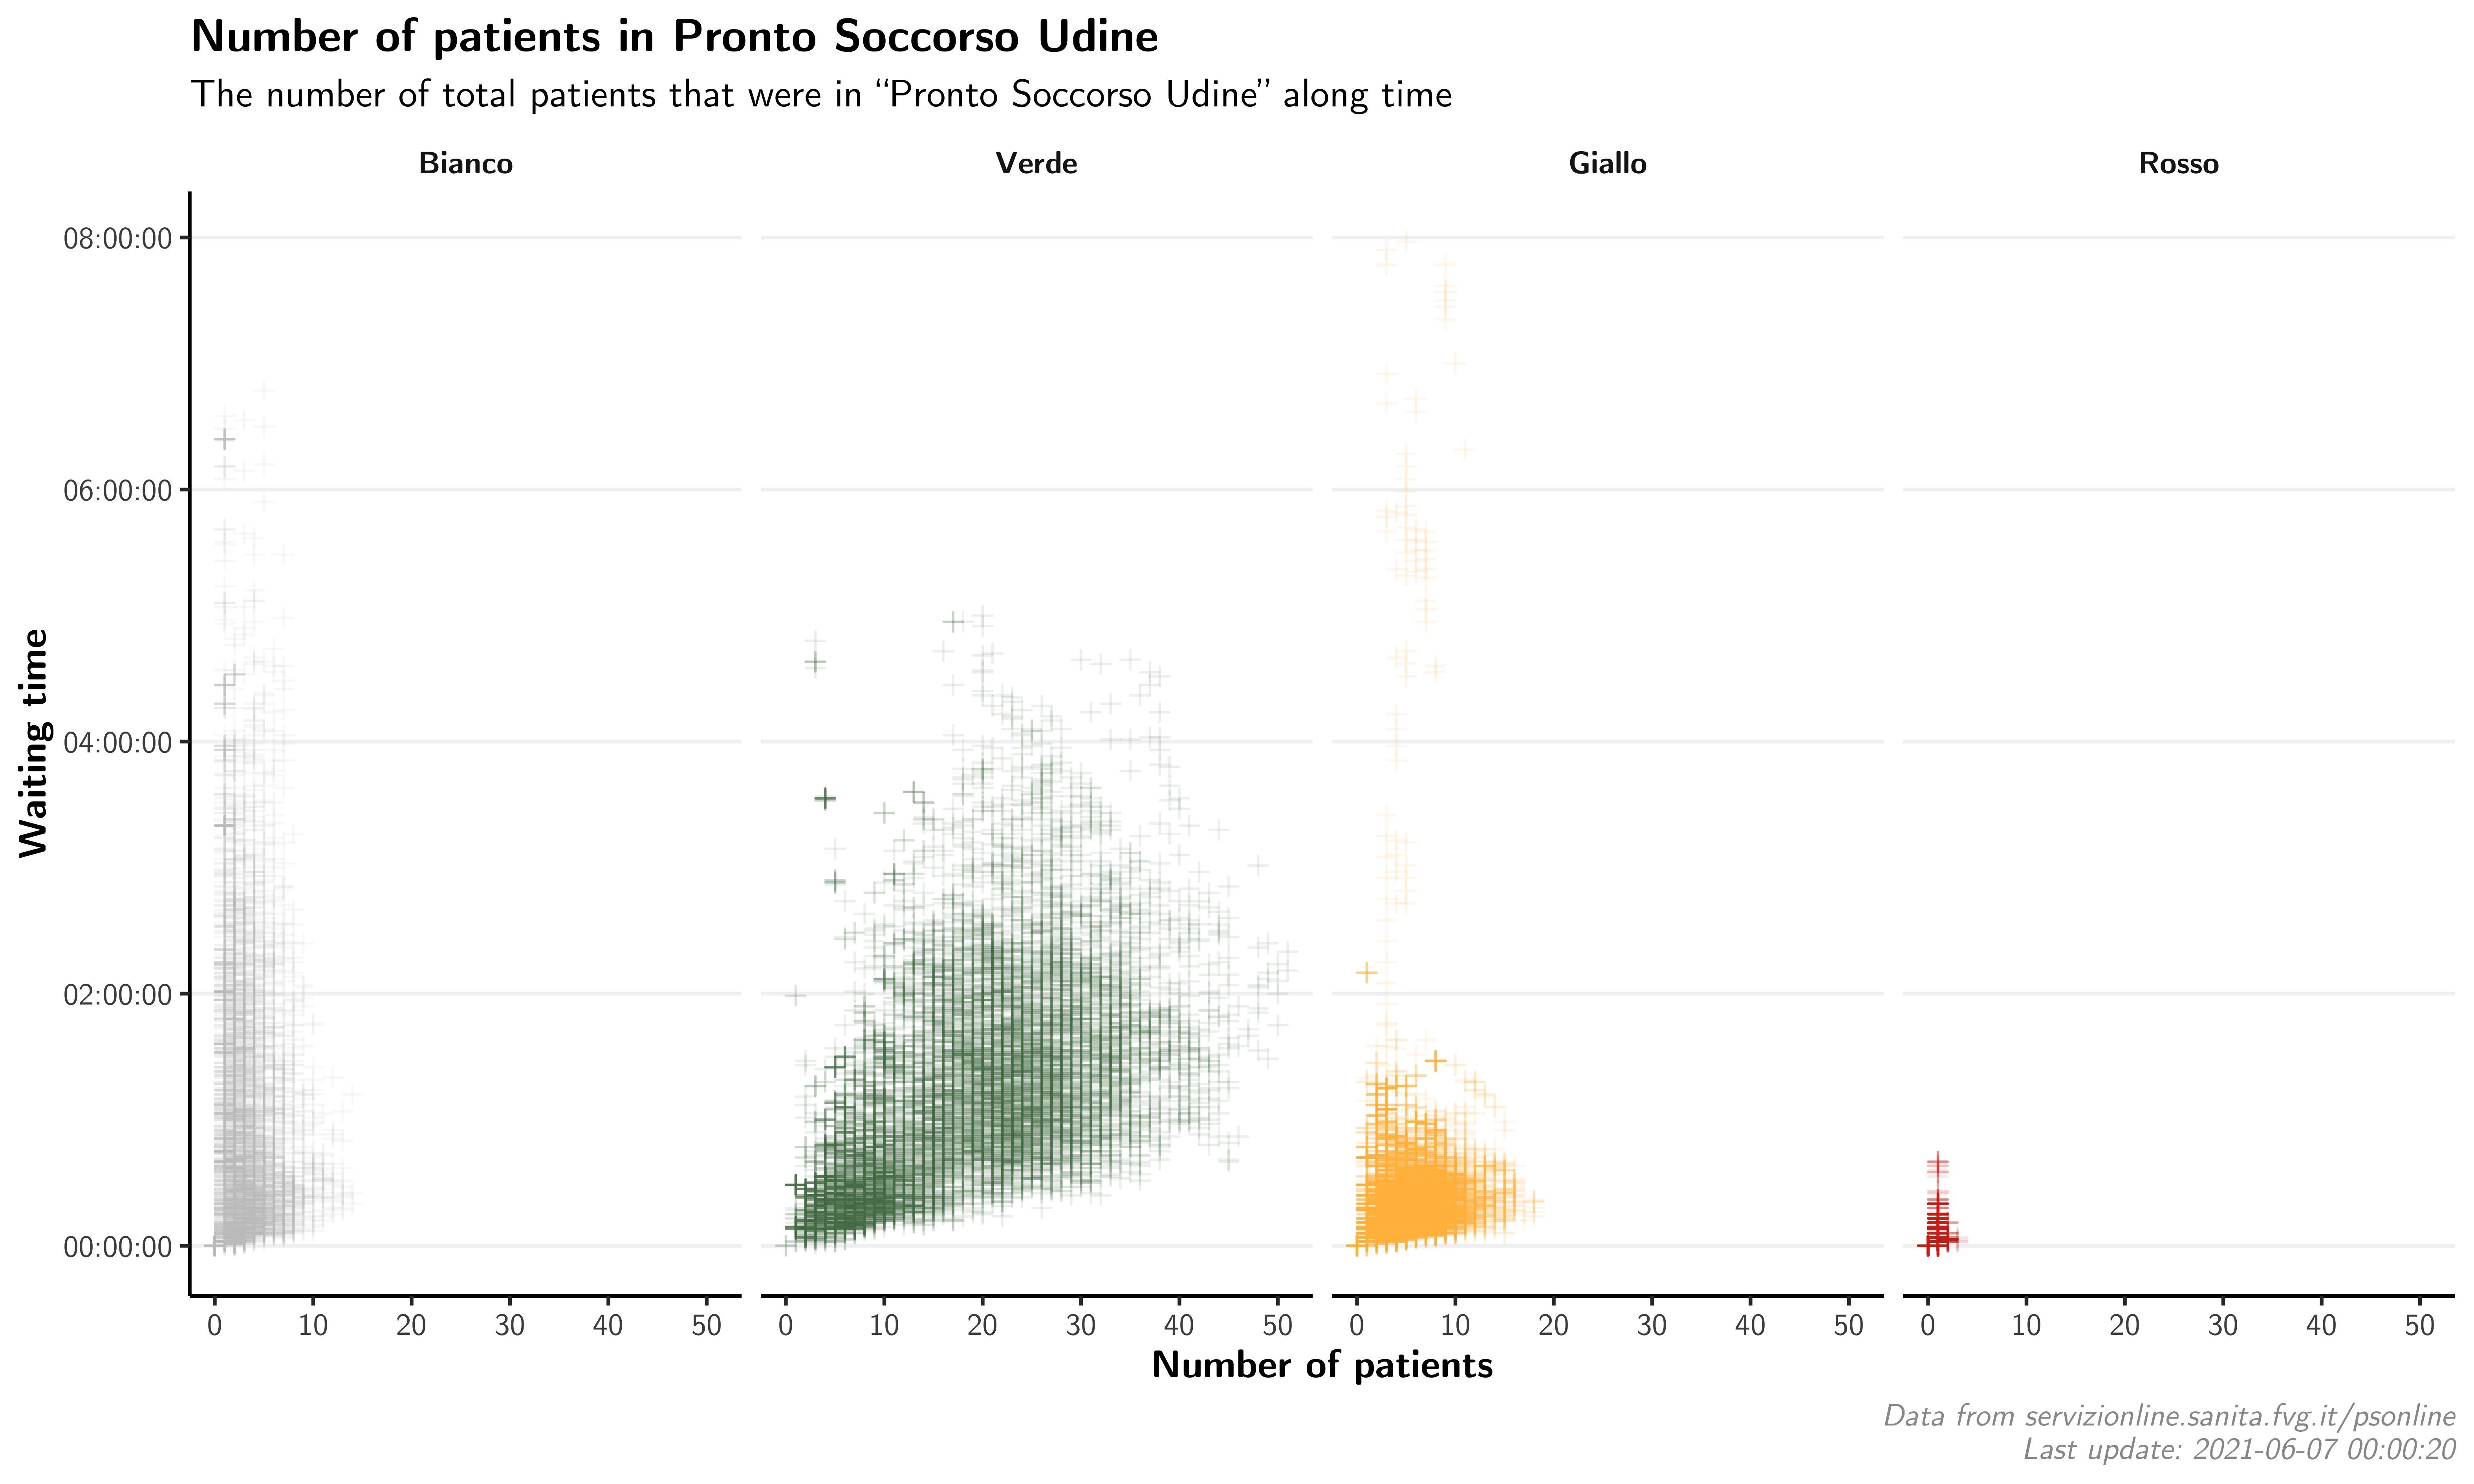
\includegraphics[width=0.75\textwidth]{../images/05_priority_scatterplot.jpg}
\end{figure}
\note{
Relativamente ai codici di priorità, potremmo ipotizzare che il tempo di attesa diminuisce quando aumenta la priorità, e il numero di pazienti diminuisce.
In questa maniera i pazienti 'Bianco' dovranno aspettare la maggior quantità di tempo, 'Verde', 'Giallo' meno, e i pazienti 'Rosso' con il tempo più basso.

Calcolando il coefficiente di Spearman tra la variabile \textit{waiting\_time} e \textit{priority} (trattata come discreta), otteniamo un valore di circa $-0.50$. Il segno meno del coefficiente ci indica che effettivamente il tempo di attesa diminuisce con l'aumentare della priorità. Il valore assoluto, però, è molto distante da $1$, e questo ci indica uno scarso legame in media tra le due variabili.

Utilizziamo la funzione di Spearman invece di quella di Pearson perché non ci aspettiamo una relazione strettamente lineare tra le variabili, ma ci chiediamo semplicemente se la funzione è monotona.

Lo scenario che ci aspettavamo è abbastanza rispettato, con una variazione sostanziale: il numero di pazienti con codice di priorità 'Bianco' è molto basso.
Al contrario, ci aspettavamo che il numero di pazienti in Pronto Soccorso aumentasse al diminuire della gravità della priorità.

Questo fenomeno può essere spiegato in diversi modi: per esempio, possiamo pensare che dopo la diffusione del COVID le persone sono più riluttanti a recarsi nei Pronto Soccorso dove possono incontrare malati gravi, se non in situazioni strettamente necessarie.}
\end{frame}

\begin{frame}
\begin{figure}
  \centering
  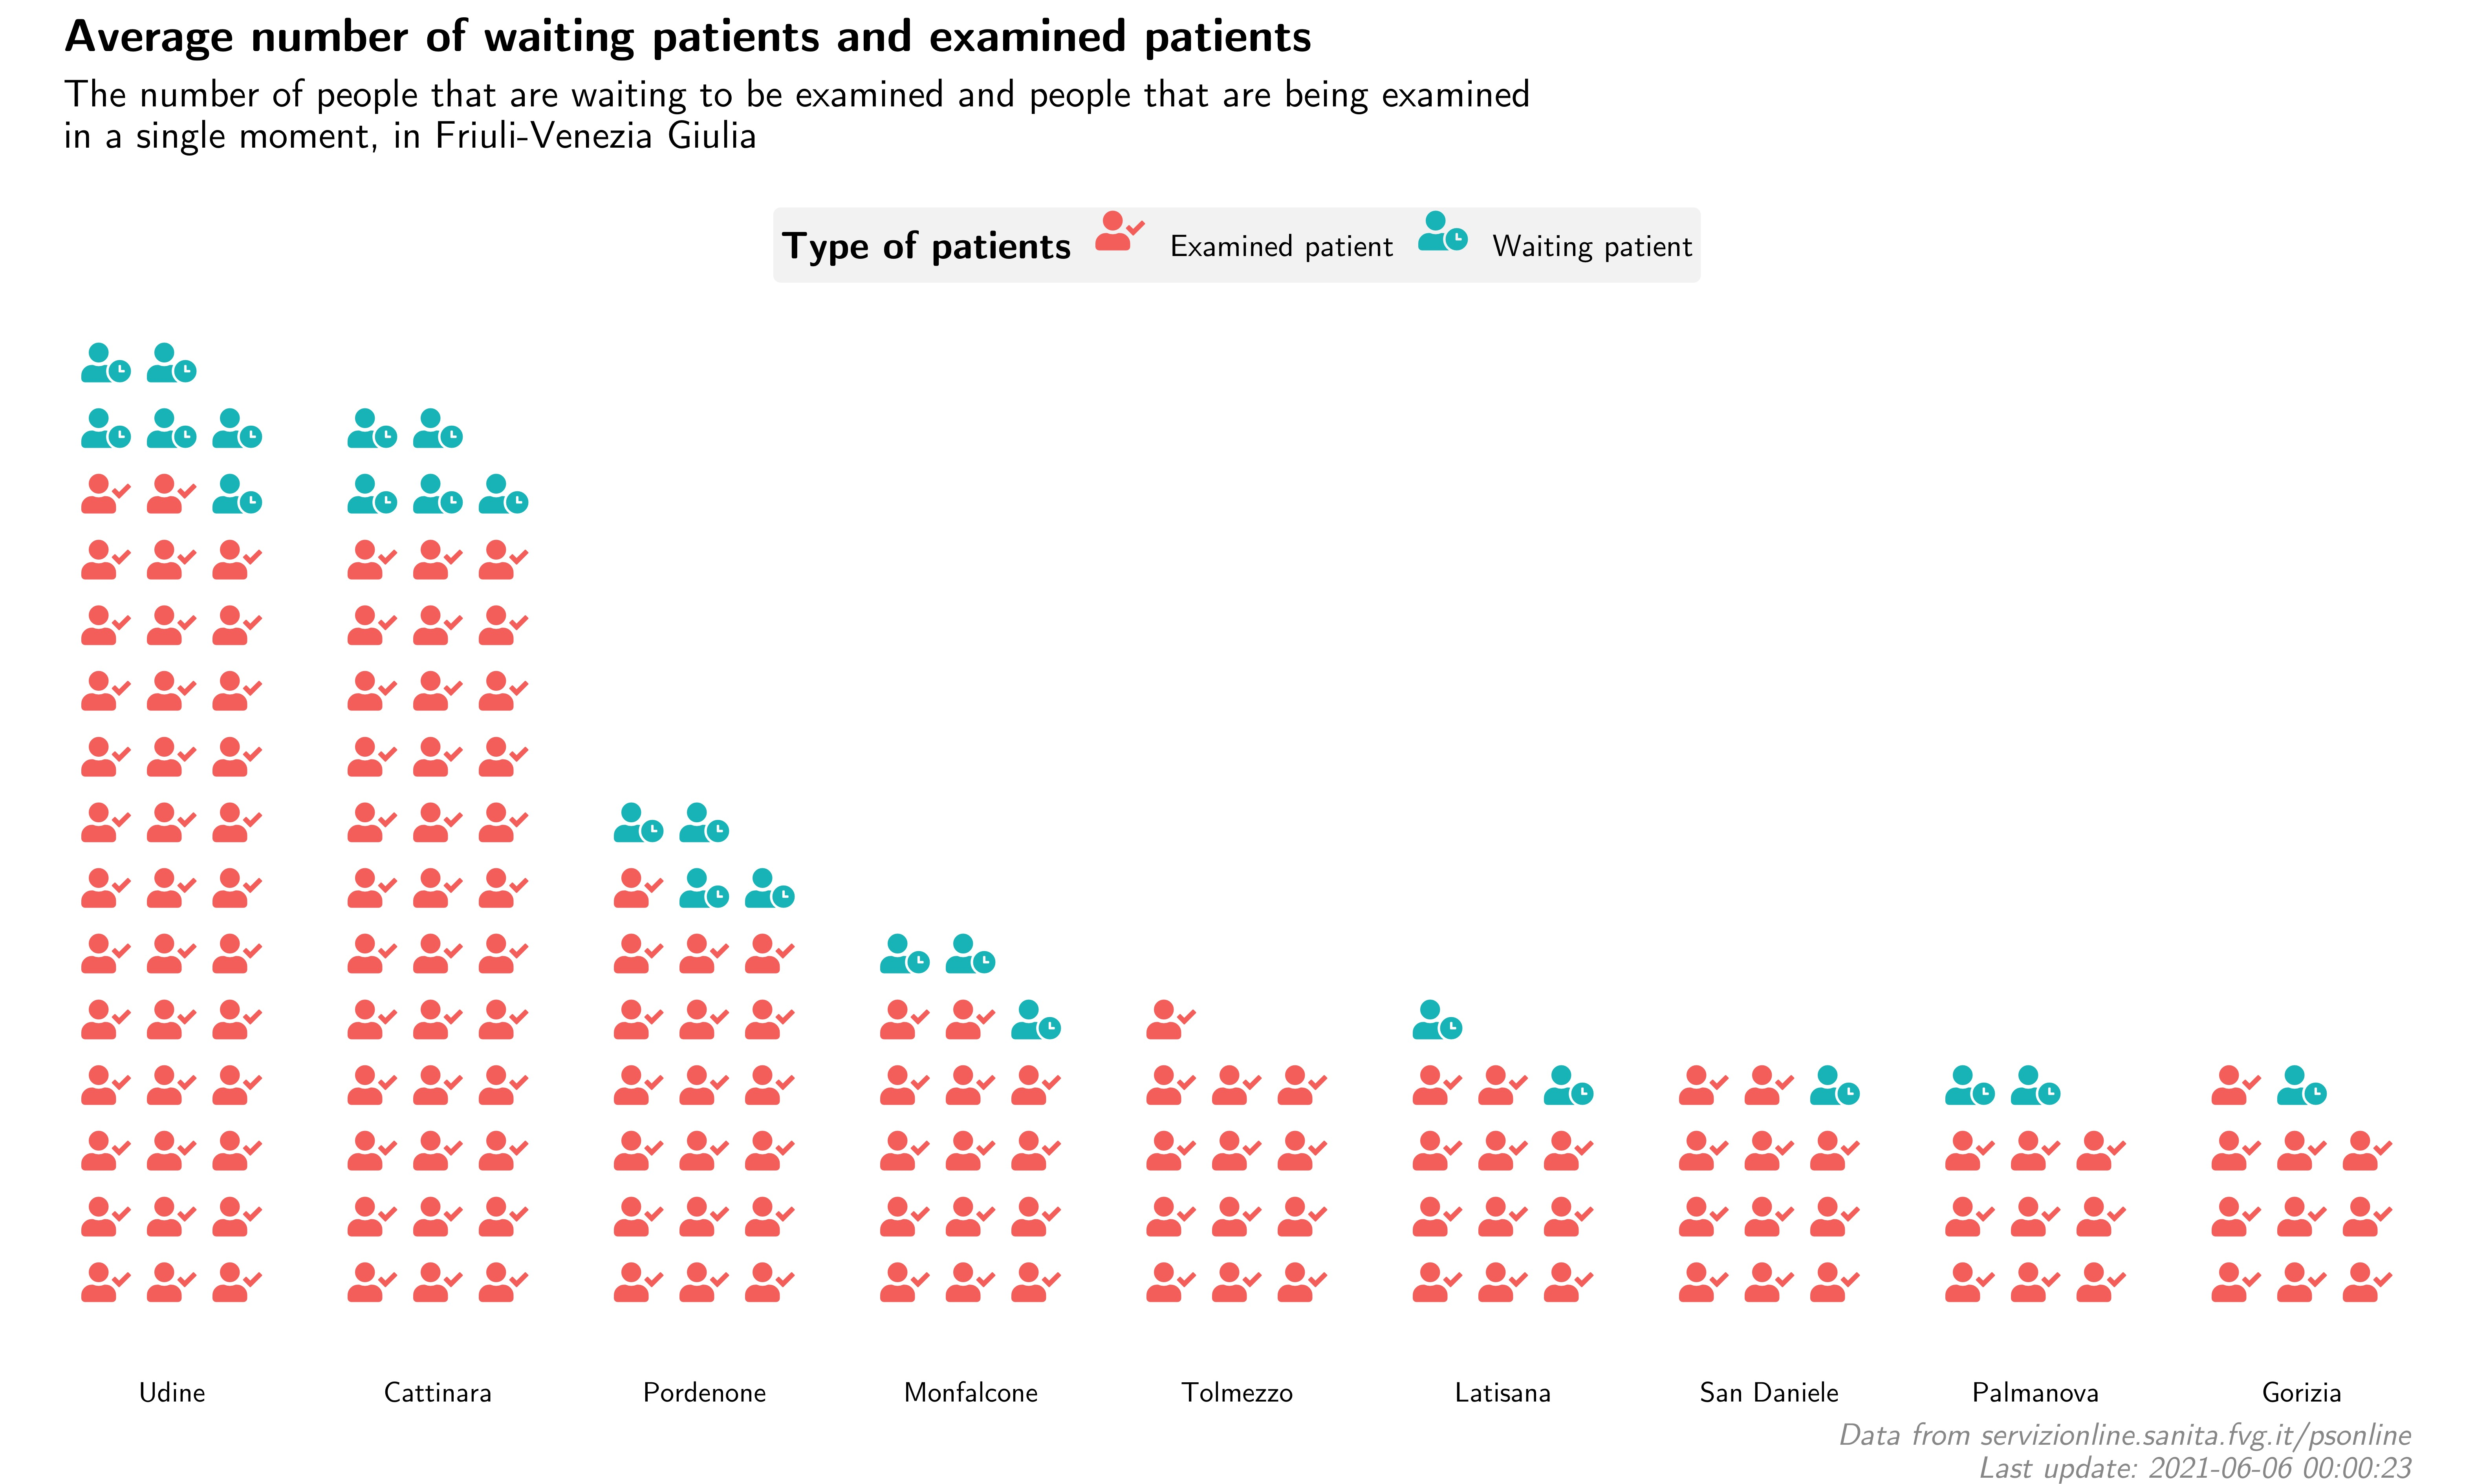
\includegraphics[width=0.75\textwidth]{../images/08_waiting-examined_waffle.jpg}
\end{figure}
\note{Da questo grafico vediamo, per i principali Pronto Soccorso della Regione (ovvero quelli con una presenza mediana di almeno 10 pazienti) qual è il rapporto tra pazienti in attesa e pazienti in esame.

}
\end{frame}

\begin{frame}
\begin{figure}
  \centering
  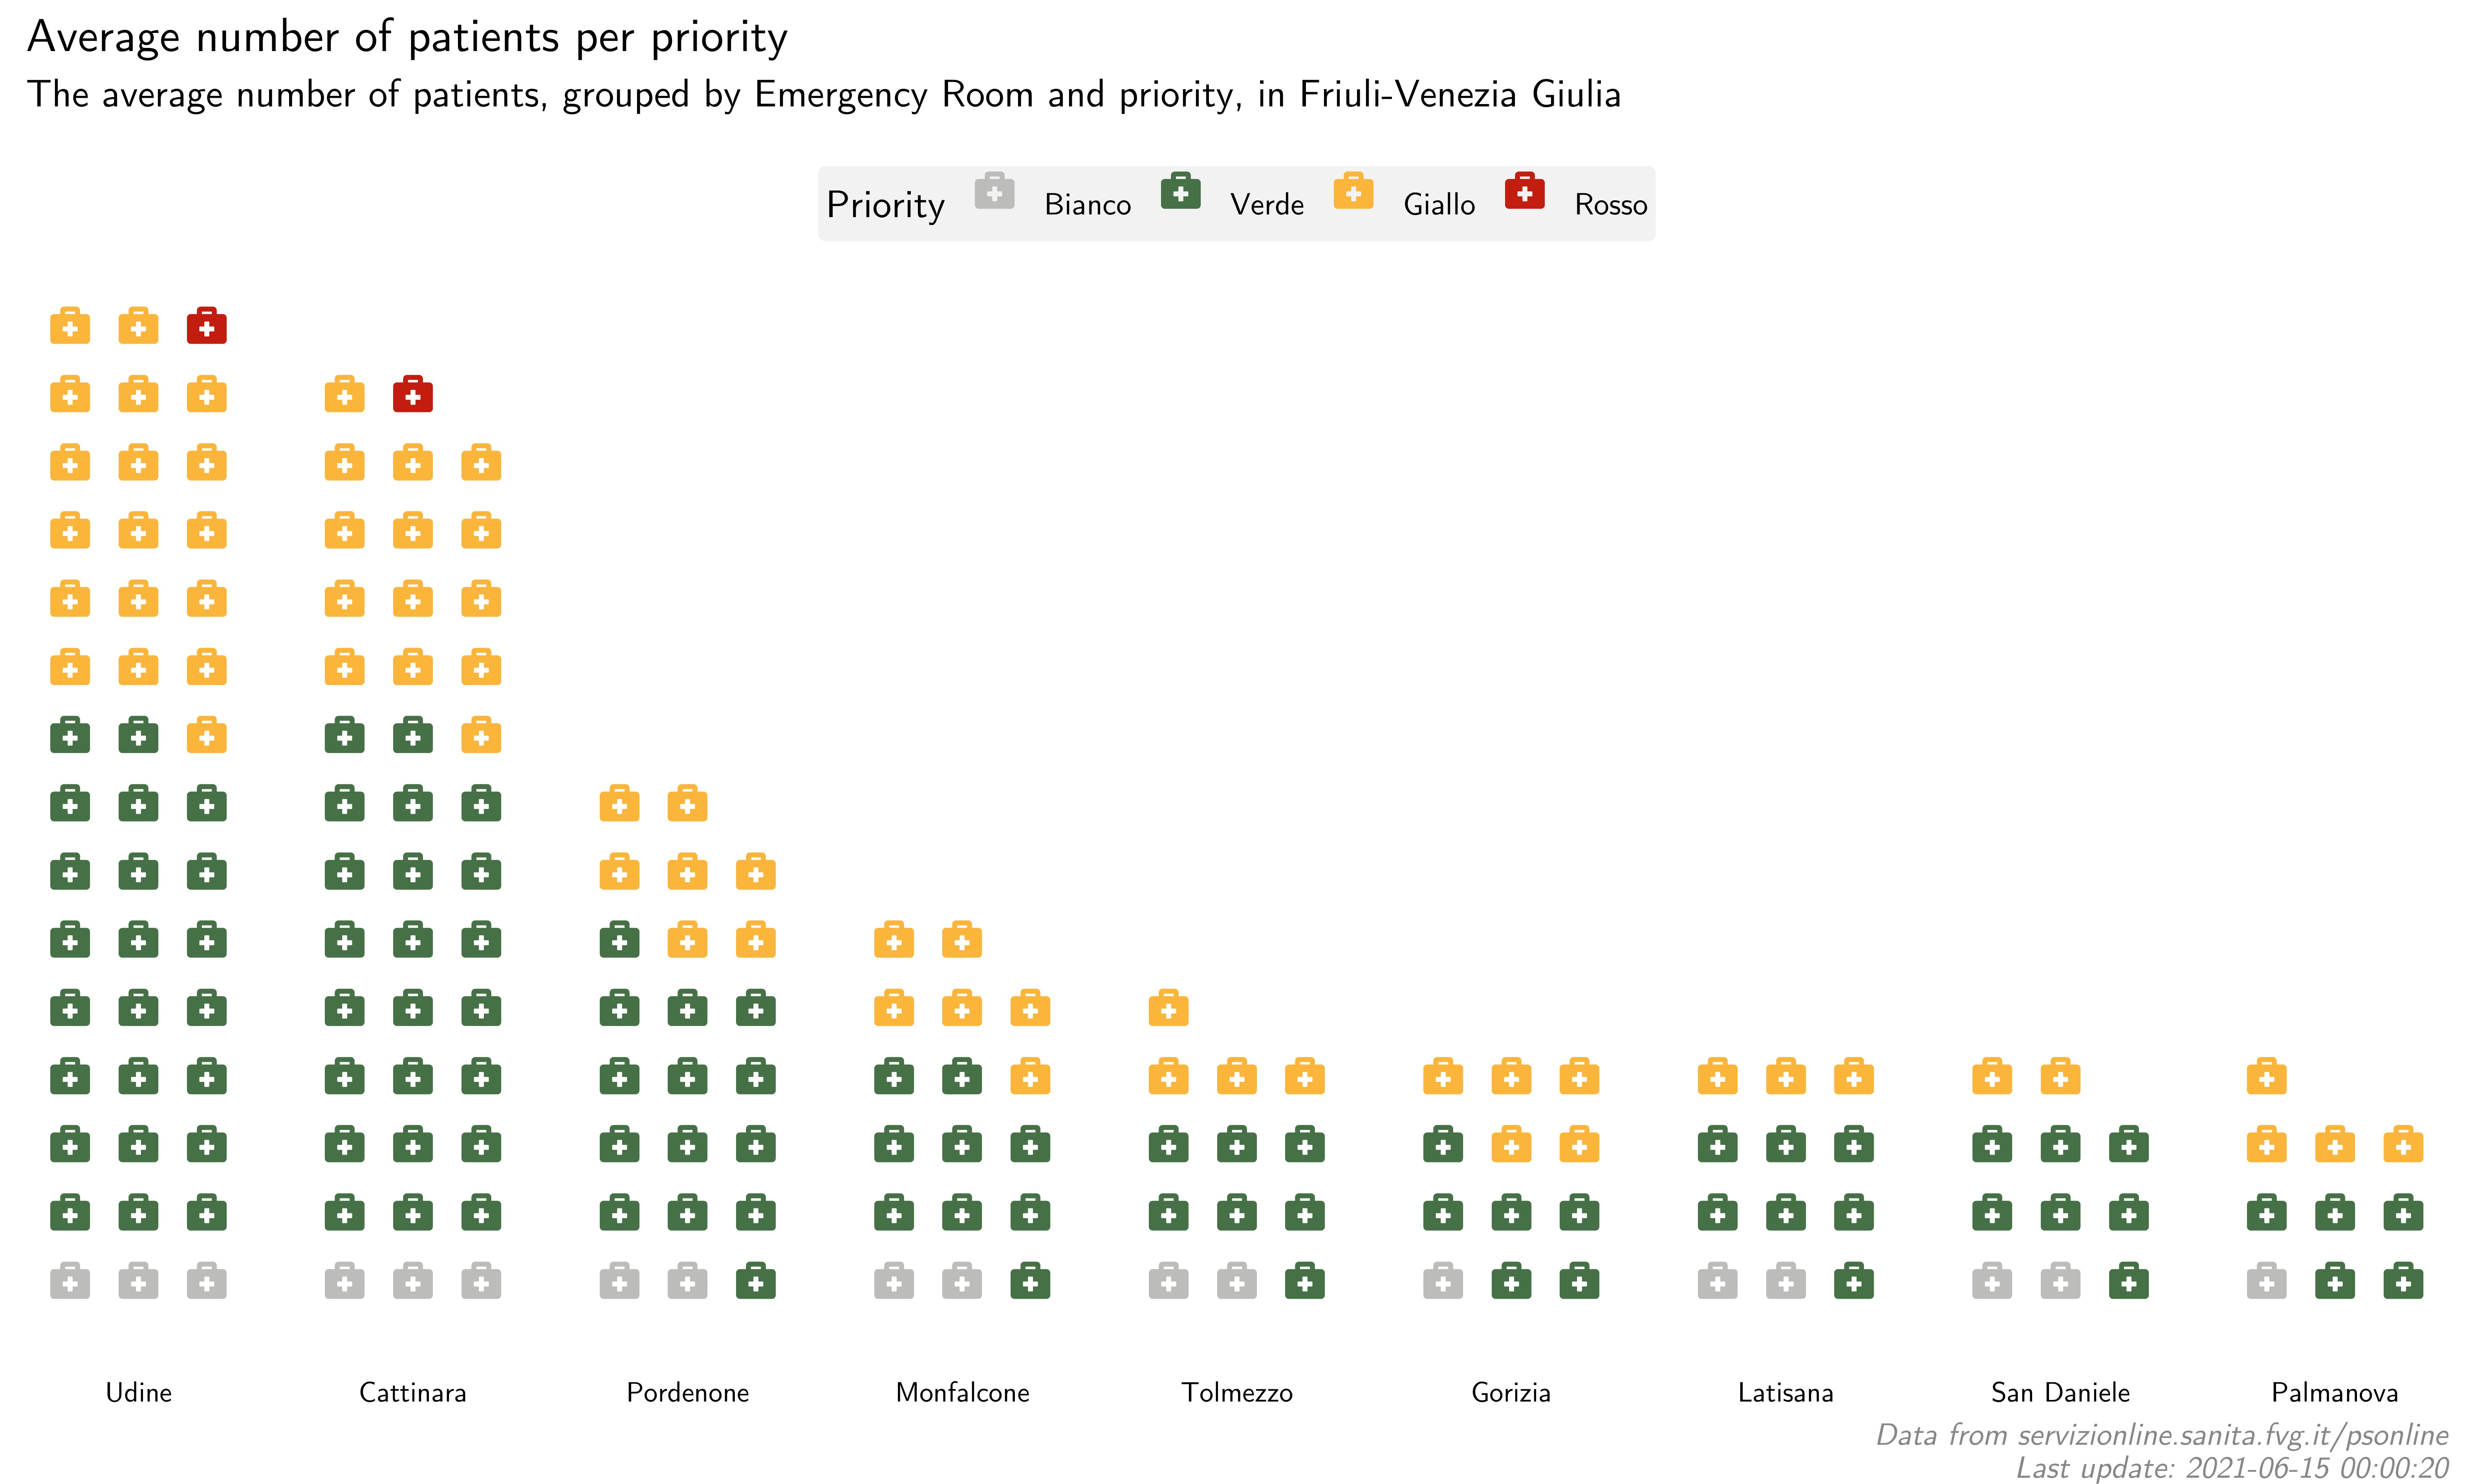
\includegraphics[width=0.75\textwidth]{../images/09_priority_waffle.jpg}
\end{figure}
\note{Il grafico in questa slide è lo stesso della slide precedente, ma stavolta i pazienti invece di essere divisi tra pazienti in attesa e pazienti in esame, sono divisi per codice di priorità.

Le osservazioni che possiamo fare sono le stesse di quelle viste in precedenza:
\begin{itemize}
	\item la maggior parte dei pazienti ha il codice verde o il codice giallo;
	\item solo i Pronto Soccorso di Udine e Cattinara hanno almeno un paziente in codice rosso in ogni istante;
\end{itemize}

}
\end{frame}

\begin{frame}

\begin{figure}
  \centering
  \href{http://uniud.enricostefanel.it/datascience/project/images/11_day-priority_bars.gif}{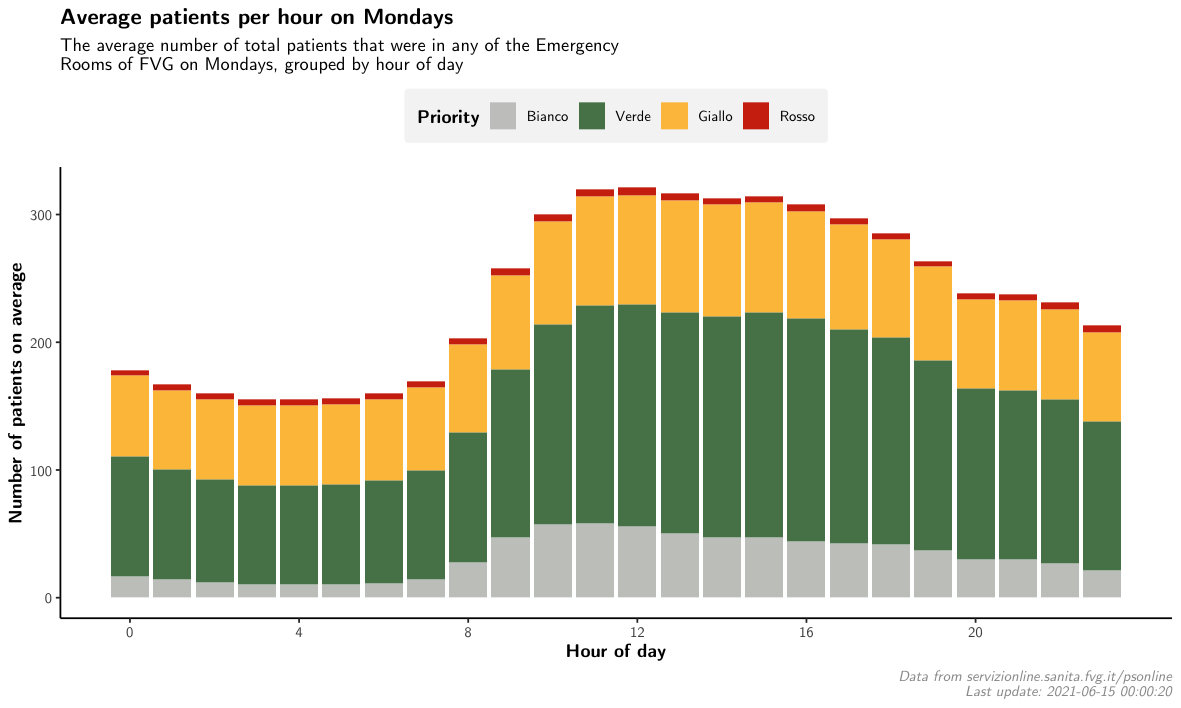
\includegraphics[width=0.75\textwidth]{../images/11_day-priority_bars.jpg}}
\end{figure}
\scriptsize \href{http://uniud.enricostefanel.it/datascience/project/images/11_day-priority_bars.gif}{\color{gray}{Click}} on the image to open the animated plot.

\note{\scriptsize Facendo \href{http://uniud.enricostefanel.it/datascience/project/images/11_day-priority_bars.gif}{\color{gray}{click}} sull'immagine si apre il grafico animato. \normalsize

Analizzando le presenze medie divise per giorno della settimana e per ora del giorno notiamo che indipendentemente dal giorno, la distribuzione di presenze nell'arco della giornata segue un andamento a curva, con massime verso mezzogiorno e prime ore del pomeriggio, e minime nella notte. Globalmente, nei weekend i Pronto Soccorso sono meno pieni, mentre il lunedì è la giornata con il carico maggiore.
}
\end{frame}

\begin{frame}
\note{Visto che il dataset è aggiornato in diretta, possiamo creare una funzione che chiamiamo \texttt{fastest\_hospital} per calcolare l'ospedale più vicino a un certo punto geografico, ottenendo anche i tempi di attesa specificando la priorità.}
Having the dataset continuously updated, we can create a function that, given as input a geographic location and an optional priority code, returns us the nearest active Emergency Room and its waiting time.

So, for instance,
\begin{itemize}
	\item if Gemona del Friuli is located at (13.14017, 46.27692), \texttt{fastest\_hospital(13.14017, 46.27692, `Giallo')} returns us \texttt{Presidio Ospedaliero di San Daniele} with waiting time about 'Giallo' priority, and
	\item \texttt{fastest\_hospital(13.43108, 46.09312)} (referred to Cividale del Friuli) returns us \texttt{Presidio Ospedaliero Universitario ``Santa Maria della Misericordia''}.
\end{itemize}
\end{frame}


\begin{frame}{Conclusions}
We used \textit{data analysis} and \textit{data visualization} to analyze attendance trends in emergency rooms in Friuli-Venezia~Giulia during this Spring.

In conclusion, it can be affirmed that the analysis carried out has not shown obvious criticalities, but on the contrary an excellent organization of the emergency system in the territory.

\note{
Abbiamo usato l'analisi dei dati e la visualizzazione dei dati per analizzare l'andamento delle presenze nei pronto soccorso del Friuli-Venezia~Giulia durante questa primavera.

In conclusione, si può affermare che l'analisi fatta non ha evidenziato evidenti criticità, ma al contrario un'ottima organizzazione del sistema di emergenza nel territorio.}

\end{frame}


\end{document}